\documentclass[convert={density=1024}]{standalone}
\usepackage{amsmath, amsthm, amsfonts,mathrsfs}
\usepackage{tikz-cd, kotex}
\usepackage{../.preamble/quiver}
\usepackage{../.preamble/Operators}
\begin{document}


% adding_extra_variables (Fiber_products-7.png)
\begin{tikzcd}
	{\Spec A[\x_1,\ldots,\x_n]} & {\Spec B[\x_1,\ldots,\x_n]} \\
	{\Spec A} & {\Spec B}
	\arrow[from=1-1, to=1-2]
	\arrow[from=1-1, to=2-1]
	\arrow[from=1-2, to=2-2]
	\arrow[from=2-1, to=2-2]
\end{tikzcd}





\end{document}

%% localizations (Affine_schemes-1.png)
\begin{tikzcd}
	{S(g)^{-1}A} & {S_g^{-1}A} \\
	{S(f)^{-1}A} & {S_f^{-1}A}
	\arrow[from=1-1, to=1-2]
	\arrow[shorten <=3pt, from=1-1, to=2-1]
	\arrow[from=1-2, to=2-2]
	\arrow[from=2-1, to=2-2]
\end{tikzcd}

%% universal_property-1 (Affine_schemes-2.png)
\begin{tikzcd}
	A & {S_f^{-1}A} \\
	& {S(f)^{-1}A}
	\arrow["{\epsilon_f}", from=1-1, to=1-2]
	\arrow["{\epsilon(f)}"', from=1-1, to=2-2]
	\arrow["{\overline{\epsilon(f)}}", from=1-2, to=2-2]
\end{tikzcd}

%% universal_property-2 (Affine_schemes-3.png)
\begin{tikzcd}
	A & {S(f)^{-1}A} \\
	& {S_f^{-1}A}
	\arrow["{\epsilon(f)}", from=1-1, to=1-2]
	\arrow["{\epsilon_f}"', from=1-1, to=2-2]
	\arrow["{\overline{\epsilon_f}}", from=1-2, to=2-2]
\end{tikzcd}

%% universal_property-3 (Affine_schemes-4.png)
\begin{tikzcd}
	A & {S(g)^{-1}A} \\
	& {S(f)^{-1}A}
	\arrow["{\epsilon(g)}", from=1-1, to=1-2]
	\arrow["{\epsilon(f)}"', from=1-1, to=2-2]
	\arrow[from=1-2, to=2-2]
\end{tikzcd}

%% universal_property-4 (Affine_schemes-5.png)
\begin{tikzcd}
	A & {S_g^{-1}A} \\
	& {S_f^{-1}A}
	\arrow["{\epsilon_g}", from=1-1, to=1-2]
	\arrow["{\epsilon_f}"', from=1-1, to=2-2]
	\arrow[from=1-2, to=2-2]
\end{tikzcd}

%% universal_property-5 (Affine_schemes-6)
\begin{tikzcd}[crossing over clearance=.5ex]
	A \\
	&{S(g)^{-1}A} &[20pt] {S_g^{-1}A} \\[15pt]
	& {S(f)^{-1}A} & {S_f^{-1}A}
	\arrow["{\epsilon(g)}"{description}, from=1-1, to=2-2]
	\arrow["{\epsilon(f)}"', curve={height=6pt},  from=1-1, to=3-2]
	\arrow["{\overline{\epsilon_g}}", from=2-2, to=2-3]
	\arrow["{\epsilon_f}"{description}, curve={height=-22pt}, crossing over, from=1-1, to=3-3, pos=.8]
	\arrow["{\epsilon_g}",  curve={height=-8pt}, from=1-1, to=2-3]
	\arrow["{\widehat{\epsilon(f)}}"', from=2-2, to=3-2]
	\arrow["{\widecheck{\epsilon_f}}", from=2-3, to=3-3]
	\arrow["{\overline{\epsilon_f}}"', from=3-2, to=3-3]
	\arrow["{\widetilde{\epsilon_f}}" description, dashed, from=2-2, to=3-3]
\end{tikzcd}

%% stalk_and_localization (Affine_schemes-7.png)
\begin{tikzcd}
	{\mathscr{O}_{\Spec A}(D(f))} & {\mathscr{O}_{\Spec A, \mathfrak{p}}} \\
	{A_f} & {A_\mathfrak{p}}
	\arrow[from=1-1, to=1-2]
	\arrow[from=1-1, to=2-1]
	\arrow[from=1-2, to=2-2]
	\arrow[from=2-1, to=2-2]
\end{tikzcd}


%% stalk_and_localization-2 (Affine_schemes-8.png)
\begin{tikzcd}
	{A_{f_j}} && {A_{f_i}} \\
	& {\displaystyle\varinjlim_{\mathfrak{p}\not\ni f}A_f} \\
	{\mathscr{O}_{\Spec A}(D(f_j))} && {\mathscr{O}_{\Spec A}(D(f_i))} \\
	& {\displaystyle \mathscr{O}_{\Spec A, \mathfrak{p}}=\varinjlim_{D(f)\ni\mathfrak{p}}\mathscr{O}_{\Spec A}(D(f))}
	\arrow[from=1-1, to=1-3]
	\arrow[from=1-1, to=2-2]
	\arrow[from=1-1, to=3-1]
	\arrow[from=1-3, to=2-2]
	\arrow[from=1-3, to=3-3]
	\arrow[from=3-1, to=3-3]
	\arrow[from=3-1, to=4-2]
	\arrow[from=3-3, to=4-2]
	\arrow[from=2-2, to=4-2, crossing over]
\end{tikzcd}

%% faithful (Affine_schemes-9.png)
\begin{tikzcd}
	&[-60pt] {\varphi_\ast\mathscr{O}_{\Spec B}(\Spec A)=\mathscr{O}_{\Spec B}(\Spec B)} && {\mathscr{O}_{\Spec B, \mathfrak{q}}} \\[30pt]
	{\mathscr{O}_{\Spec A}(\Spec A)} && {\mathscr{O}_{\Spec A, \varphi(\mathfrak{q})}} \\
	& B && {B_\mathfrak{q}} \\[30pt]
	A && {A_{\varphi(\mathfrak{q})}}
	\arrow[from=1-2, to=1-4]
	\arrow[from=1-2, to=3-2]
	\arrow[from=1-4, to=3-4]
	\arrow["{\varphi^\sharp(\Spec A)}"{description}, from=2-1, to=1-2]
	\arrow[from=2-1, to=4-1]
	\arrow["{\varphi^\sharp_{\mathfrak{q}}}"{description}, from=2-3, to=1-4]
	\arrow[from=3-2, to=3-4]
	\arrow["\phi"{description}, from=4-1, to=3-2]
	\arrow[from=4-1, to=4-3]
	\arrow["{\phi_\mathfrak{q}}"{description}, from=4-3, to=3-4]
	\arrow[from=2-1, to=2-3, crossing over]
	\arrow[from=2-3, to=4-3, crossing over]
\end{tikzcd}

%% commuting_square (Affine_schemes-10.png)
\begin{tikzcd}
	{\mathscr{O}_{\Spec A, \varphi(\mathfrak{q})}} & {\mathscr{O}_{\Spec B, \mathfrak{q}}} \\
	{A_{\varphi(\mathfrak{q})}} & {B_\mathfrak{q}}
	\arrow["{\varphi_\mathfrak{q}^\sharp}", from=1-1, to=1-2]
	\arrow[from=1-1, to=2-1]
	\arrow[from=1-2, to=2-2]
	\arrow["{\phi_\mathfrak{q}}"', from=2-1, to=2-2]
\end{tikzcd}

%% adjoint (Affine_schemes-11.png)
\begin{tikzcd}
	&[-30pt] {\varphi_\ast\mathscr{O}_{X}(\Spec A)=\mathscr{O}_{X}(X)} && {\mathscr{O}_{X, x}} \\[30pt]
	{\mathscr{O}_{\Spec A}(\Spec A)} && {\mathscr{O}_{\Spec A, \varphi(x)}} \\[30pt]
	A && {A_{\varphi(x)}}
	\arrow[from=1-2, to=1-4]
	\arrow["{\varphi^\sharp(\Spec A)}"{description}, from=2-1, to=1-2]
	\arrow[from=2-1, to=3-1]
	\arrow["{\varphi^\sharp_x}"{description}, from=2-3, to=1-4]
	\arrow[from=3-1, to=1-2]
	\arrow[from=3-1, to=3-3]
	\arrow[from=2-1, to=2-3, crossing over]
	\arrow[from=2-3, to=3-3, crossing over]
	\arrow[from=3-3, to=1-4, dashed]
\end{tikzcd}


%% decomposition (Schemes-1.png)
\begin{tikzcd}
	\Spec A_f\rar["\Spec\epsilon"]\drar[sloped, swap, "\sim" above]\drar["\Spec\epsilon\vert^{D(f)}" {below, xshift=-12pt, yshift=-3pt}]&\Spec A\\
	&D(f)\uar[hook, "\iota" right]
\end{tikzcd}

%line_with_two_origins (Schemes-2.png)
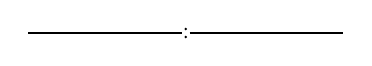
\begin{tikzpicture}
	\draw (-2,0)--(-.05,0);
	\draw (.05,0)--(2,0);
	\fill (0,0.05) circle[radius=.5pt];
	\fill (0,-.05) circle[radius=.5pt];
\end{tikzpicture}

%projective_line (Schemes-3.png)
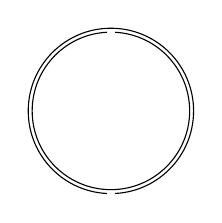
\begin{tikzpicture}
	\draw (0,0) circle[radius=1];
	\draw (0,0) circle[radius=1.05];
	\draw[white, very thick] (-.05,1)--(.05,1);
	\draw[white, very thick] (-.05,-1.05)--(.05,-1.05);
\end{tikzpicture}


%% stereographic_projection (Projective_schemes-1.png)
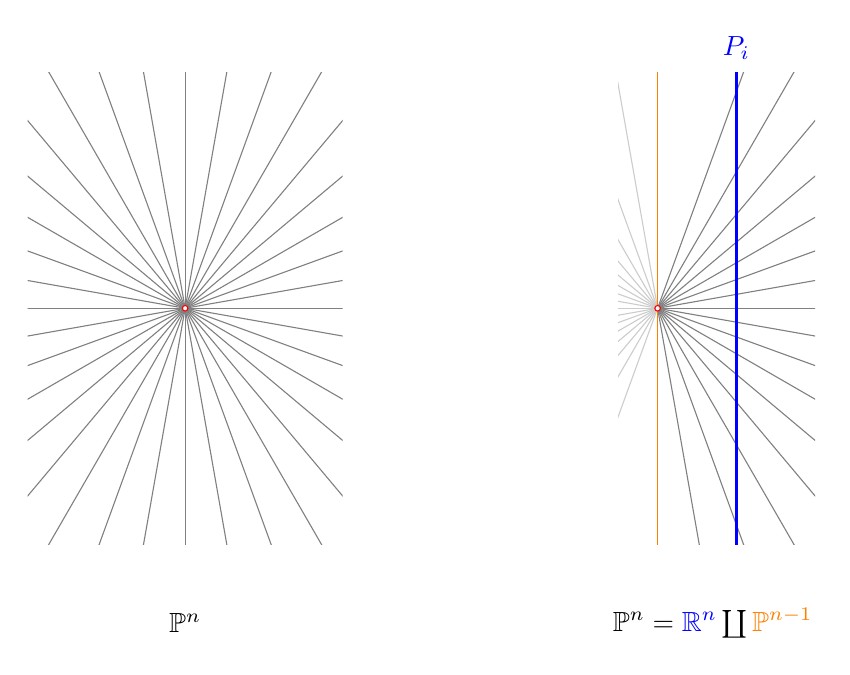
\begin{tikzpicture}
	\begin{scope}
		\clip (-2,-3) rectangle (2,3);
		\foreach \t in {-90,-80,...,80}{
			\draw[gray] (\t:0)--(\t:20);
			\draw[gray] (\t:-20)--(\t:0);
		}
		\filldraw[draw=red, fill=white] (0,0) circle[radius=1pt];
	\end{scope}
	\draw (0,-4) node{$\mathbb{P}^n$};
	\begin{scope}[shift={(6,0)}]
		\clip (-.5,-3) rectangle (2,3);
		\foreach \t in {-80,-70,...,70}{
			\draw[gray] (\t:0)--(\t:20);
			\draw[gray!40] (\t:-20)--(\t:0);
		}
		\draw[orange] (0,-4)--(0,4);
		\draw[blue, very thick] (1,-4)--(1,4);
		\filldraw[draw=red, fill=white] (0,0) circle[radius=1pt];
	\end{scope}
	\draw[blue] (7,3.3) node{$P_i$};
	\draw (6.7,-4) node{$\mathbb{P}^n={\color{blue}\mathbb{R}^n}\coprod {\color{orange}\mathbb{P}^{n-1}}$};
\end{tikzpicture}

% finite_type_morphism (Properties_of_scheme_morphisms-1.png)
\begin{tikzpicture}
	\draw[blue] (-2,0) -- (2,0);
	\fill[blue!30] (-2,1) rectangle (2,5);
	\fill (-1,0) circle [radius=2pt];
	\draw[thick] (-1,1) -- (-1,5);
	\draw[-{stealth}] (0,0.8) -- (0,0.2);
	\draw (4.5,3) node{$\mathbb{A}^2_\Bbbk\cong \Spec \Bbbk[\x,\y]\cong \Spec \Bbbk[\x][\y]$};
	\draw (4,0) node{$\mathbb{A}^1_\Bbbk\cong \Spec \Bbbk[\x]$};
\end{tikzpicture}

% finite_morphism (Properties_of_scheme_morphisms-2.png)
\begin{tikzpicture}
	\draw (-.1,-4)--(4.9,-4) node[right]{$\mathbb{A}^1_\Bbbk\cong \Spec \Bbbk[\x]$};
	\draw[domain=0:2.2] plot (\x^2,\x)node[right]{$\Spec \Bbbk[\x,\y]/(\y^2-\x)$};
	\draw[domain=0:2.2] plot (\x^2,-\x);
	\fill (4,-4) circle[radius=2pt];
	\draw[dashed, gray] (4,2)--(4,-4); 
	\draw[-{stealth}] (2.5,-2.5) -- (2.5,-3.5);
	\fill[red] (4,2) circle[radius=2pt];
	\fill[red] (4,-2) circle[radius=2pt];
\end{tikzpicture}


%% fiber_diagram (Fiber_products-1.png)
\begin{tikzcd}
	{X\times_SY} & Y \\
	X & S
	\arrow["{\rho_Y}", from=1-1, to=1-2]
	\arrow["{\rho_X}"', from=1-1, to=2-1]
	\arrow["{\varphi_Y}", from=1-2, to=2-2]
	\arrow["{\varphi_X}"', from=2-1, to=2-2]
\end{tikzcd}

%% universal_property (Fiber_products-2.png)
\begin{tikzcd}
	Z \\
	& {X\times_SY} & Y \\
	& X & S
	\arrow["\psi"{description}, dashed, from=1-1, to=2-2]
	\arrow["{\psi_Y}", curve={height=-12pt}, from=1-1, to=2-3]
	\arrow["{\psi_X}"', curve={height=12pt}, from=1-1, to=3-2]
	\arrow["{\rho_Y}", from=2-2, to=2-3]
	\arrow["{\rho_X}"', from=2-2, to=3-2]
	\arrow["{\varphi_Y}", from=2-3, to=3-3]
	\arrow["{\varphi_X}"', from=3-2, to=3-3]
\end{tikzcd}

% open_subscheme (Fiber_products-3.png)
\begin{tikzcd}
	{\varphi^{-1}(U)} & U \\
	Y & Z
	\arrow["{\varphi\vert^U}", from=1-1, to=1-2]
	\arrow["{\iota'}"', from=1-1, to=2-1]
	\arrow["\iota", from=1-2, to=2-2]
	\arrow["\varphi"', from=2-1, to=2-2]
\end{tikzcd}

%% open_fiber_product-1 (Fiber_products-4.png)
\begin{tikzcd}
	{X\times_SY} & Y \\
	X & S
	\arrow["{\rho_Y}", from=1-1, to=1-2]
	\arrow["{\rho_X}"', from=1-1, to=2-1]
	\arrow["\lrcorner"{anchor=center, pos=0.125}, draw=none, from=1-1, to=2-2]
	\arrow["{\varphi_Y}", from=1-2, to=2-2]
	\arrow["{\varphi_X}"', from=2-1, to=2-2]
\end{tikzcd}

%% open_fiber_product-2 (Fiber_products-5.png)
\begin{tikzcd}
	& {Y'} \\
	{X\times_SY} & Y
	\arrow[hook, from=1-2, to=2-2]
	\arrow["{\rho_Y}"', from=2-1, to=2-2]
\end{tikzcd}

%% magic_square (Fiber_products-6.png)
\begin{tikzcd}
	{\rho_Y^{-1}(Y')} & {Y'} \\
	{X\times_SY} & Y \\
	X & S
	\arrow[from=1-1, to=1-2]
	\arrow[from=1-1, to=2-1]
	\arrow["\lrcorner"{anchor=center, pos=0.125}, draw=none, from=1-1, to=2-2]
	\arrow[hook, from=1-2, to=2-2]
	\arrow[from=2-1, to=2-2]
	\arrow[from=2-1, to=3-1]
	\arrow["\lrcorner"{anchor=center, pos=0.125}, draw=none, from=2-1, to=3-2]
	\arrow[from=2-2, to=3-2]
	\arrow[from=3-1, to=3-2]
\end{tikzcd}




















% multiplicity (Algebraic_varieties-1.png)
\begin{tikzpicture}
	\draw (-2,0)--(2,0);
	\draw[domain=-2:0, variable=\x] plot({\x}, {-\x^2});
	\draw[domain=0:2, variable=\x] plot({\x}, {\x^2});
	\fill (0,0) circle[radius=2pt];
	\draw (-9,2)--(-5,2);
	\draw (-7,0) -- (-7,4);
	\fill (-7,2) circle[radius=2pt];
	\draw (-7,-.5) node{$V(x,y)$};
	\draw (0,-.5) node{$V(y, y-x^2)$};
\end{tikzpicture}

% presheaf_morphism (Presheaves-1.png)
\begin{tikzcd}
	{\mathcal{F}(V)} & {\mathcal{G}(V)} \\
	{\mathcal{F}(U)} & {\mathcal{G}(U)}
	\arrow["{\phi(V)}", from=1-1, to=1-2]
	\arrow["{\phi(U)}"', from=2-1, to=2-2]
	\arrow[from=1-2, to=2-2]
	\arrow[from=1-1, to=2-1]
\end{tikzcd}

% presheaf_kernel-1 (Presheaves-2.png)
\begin{tikzcd}
	0 & {\ker \phi(V)} & {\mathcal{F}(V)} & {\mathcal{G}(V)} \\
	0 & {\ker\phi(U)} & {\mathcal{F}(U)} & {\mathcal{G}(U)}
	\arrow[from=1-1, to=1-2]
	\arrow[from=1-2, to=1-3]
	\arrow[from=1-3, to=1-4]
	\arrow[from=2-3, to=2-4]
	\arrow[from=2-2, to=2-3]
	\arrow[from=2-1, to=2-2]
	\arrow[from=1-3, to=2-3]
	\arrow[from=1-4, to=2-4]
	\arrow[dashed, from=1-2, to=2-2]
\end{tikzcd}

% presheaf_kernel-2 (Presheaves-3.png)
\begin{tikzcd}
	0 & {\ker\phi(W)} & {\mathcal{F}(W)} & {\mathcal{G}(W)} \\
	0 & {\ker \phi(V)} & {\mathcal{F}(V)} & {\mathcal{G}(V)} \\
	0 & {\ker\phi(U)} & {\mathcal{F}(U)} & {\mathcal{G}(U)}
	\arrow[from=2-1, to=2-2]
	\arrow[from=2-2, to=2-3]
	\arrow[from=2-3, to=2-4]
	\arrow[from=3-3, to=3-4]
	\arrow[from=3-2, to=3-3]
	\arrow[from=3-1, to=3-2]
	\arrow[from=2-3, to=3-3]
	\arrow[from=2-4, to=3-4]
	\arrow[dashed, from=2-2, to=3-2]
	\arrow[from=1-2, to=1-3]
	\arrow[from=1-3, to=1-4]
	\arrow[from=1-4, to=2-4]
	\arrow[from=1-3, to=2-3]
	\arrow[dashed, from=1-2, to=2-2]
	\arrow[from=1-1, to=1-2]
	\arrow[curve={height=45pt}, dashed, from=1-2, to=3-2, crossing over]
\end{tikzcd}

% universal_property_of_sheafification (Sheaves-1.png)
\begin{tikzcd}
	{\mathcal{F}} & {\mathcal{F}^\dagger} \\
	& {\mathcal{G}}
	\arrow[from=1-1, to=2-2]
	\arrow[from=1-1, to=1-2]
	\arrow[dashed, from=1-2, to=2-2]
\end{tikzcd}


% counterexamples_connectedness/irreducibility (Properties_of_schemes-1.png)
\begin{tikzpicture}
	\draw[gray!50] (-1,0)--(2,0);
	\draw (0,-1)--(0,1);
	\draw (1,-1)--(1,1);
	\draw (4,0)--(6,0);
	\draw (5,-1)--(5,1);
	\draw (5,-1.5) node{$Z(\mathrm{x}\mathrm{y})$};
	\draw (.5,-1.5) node{$Z(\mathrm{x}(\mathrm{x}-1))$};
\end{tikzpicture}

% counterexamples_reducedness (Properties_of_schemes-2.png)
\begin{tikzpicture}
	\draw[domain=-2:0, variable=\x] plot({\x}, {-\x^2});
	\draw[domain=0:2, variable=\x] plot({\x}, {\x^2});
	\draw (0,-.5) node{$Z(\mathrm{y}-\mathrm{x}^2)$};
\end{tikzpicture}




% fiber_product (Properties_of_schemes-5.png)
\begin{tikzcd}
	W \\
	& {X\times_ZY} & Y \\
	& X & Z
	\arrow[dashed, from=1-1, to=2-2]
	\arrow["{q'}", curve={height=-6pt}, from=1-1, to=2-3]
	\arrow["{p'}"', curve={height=6pt}, from=1-1, to=3-2]
	\arrow["q", from=2-2, to=2-3]
	\arrow["p"', from=2-2, to=3-2]
	\arrow["g", from=2-3, to=3-3]
	\arrow["f"', from=3-2, to=3-3]
\end{tikzcd}

% diagonal_morphism (Valuative_criteria-1.png)
\begin{tikzcd}
	{X} \\
	& {X\times_YX} & X \\
	& X & Y
	\arrow[dashed, from=1-1, to=2-2]
	\arrow[curve={height=-6pt}, Rightarrow, no head, from=1-1, to=2-3]
	\arrow[curve={height=6pt}, Rightarrow, no head, from=1-1, to=3-2]
	\arrow[from=2-2, to=2-3]
	\arrow[from=2-2, to=3-2]
	\arrow["f", from=2-3, to=3-3]
	\arrow["f"', from=3-2, to=3-3]
\end{tikzcd}

% valuative_criterion_for_separatedness (Valuative_criteria-2.png)
\begin{tikzcd}
	{\Spec K} & X \\
	{\Spec R} & Y
	\arrow[from=1-1, to=1-2]
	\arrow[from=1-1, to=2-1]
	\arrow["f", from=1-2, to=2-2]
	\arrow[dashed, from=2-1, to=1-2]
	\arrow[from=2-1, to=2-2]
\end{tikzcd}

\begin{tikzcd}
	{\Spec K} & X \\
	{\Spec R} & Y
	\arrow[from=1-1, to=1-2]
	\arrow[from=1-1, to=2-1]
	\arrow["f", from=1-2, to=2-2]
	\arrow[dashed, from=2-1, to=1-2]
	\arrow[from=2-1, to=2-2]
\end{tikzcd}

\begin{tikzcd}
	X & A \\
	B & C
	\arrow["a"', from=1-2, to=1-1]
	\arrow["b", from=2-1, to=1-1]
	\arrow["f"', from=2-2, to=1-2]
	\arrow["g", from=2-2, to=2-1]
\end{tikzcd}
